% /home/raffael/Documents/Nextcloud/Hobbies/SpaceTeam/LiquidCan/documentation.tex
\documentclass[11pt,a4paper]{article}
\usepackage[margin=25mm]{geometry}
\usepackage{lmodern}
\usepackage[T1]{fontenc}
\usepackage[utf8]{inputenc}
\usepackage{microtype}
\usepackage{booktabs}
\usepackage{array}
\usepackage{tabularx}
\usepackage{longtable}
\usepackage{hyperref}
\usepackage{caption}
\usepackage{float}
\usepackage{tikz}
\usetikzlibrary{calc, shapes.geometric, arrows.meta, positioning, fit}
\usepackage{listings}
\usepackage{xcolor}
\usepackage{bytefield}

\hypersetup{
    colorlinks=true,
    linkcolor=blue,
    urlcolor=blue,
    pdftitle={CAN Protocol Documentation Template},
    pdfauthor={},
}

% Listings for C code
\lstset{
    language=C,
    basicstyle=\ttfamily\small,
    keywordstyle=\color{blue}\bfseries,
    commentstyle=\color{gray}\itshape,
    stringstyle=\color{red},
    showstringspaces=false,
    tabsize=2,
    breaklines=true,
    numbers=left,
    numberstyle=\tiny,
    frame=single,
    captionpos=b
}

% Custom command for register-style byte field documentation using bytefield package
% This creates a register layout similar to STM32/FDCAN documentation style
\newcommand{\regfield}[3]{%
    % #1 = byte(s), #2 = field name, #3 = description
    \item \textbf{Byte(s) #1: \texttt{#2}} -- #3
}
\newcommand{\todo}[1]{\textcolor{red}{\textbf{TODO:} #1}}
\title{LiquidCan Protocol Documentation}
\author{SpaceTeam}
\date{\today}

\begin{document}


% Header/Cover Page
\thispagestyle{empty}
\begin{center}
\vspace*{2cm}

{\Huge \textbf{LiquidCan Protocol Documentation}}

\vspace{1cm}

\vspace{0.5cm}

{\large for Distributed Embedded Systems\\ at the TU Wien Space Team}


\begin{figure}[H]
    \centering
    \includegraphics[scale=0.35]{images/SpaceTeamLogo.png}
\end{figure}
\vspace{7cm}

{\large TU Wien Space Team}

\vspace{1cm}

{\large Version 0.1}

\vspace{0.5cm}

{\large \today}

\vfill

\end{center}

\clearpage

% Version History Table
\section*{Version History}
\begin{center}
\begin{longtable}{c l p{8cm} l}
\toprule
\textbf{Version} & \textbf{Date} & \textbf{Changes} & \textbf{Author} \\
\midrule
0.1 & 2025-12-12 & Initial protocol specification & Raffael Rott \\
\midrule
 &  &  &  \\
\midrule
 &  &  &  \\
\bottomrule
\end{longtable}
\end{center}

\clearpage

\tableofcontents
\vspace{6mm}

\clearpage

\section{Purpose and Scope}
% TODO: Describe the purpose of the LiquidCan protocol
% Nodes involved:
% Expected CAN bitrate(s):
% Error handling policy:
% Versioning scheme:
% Interoperability constraints:
The purpose of the LiquidCan protocol is to serve at the heart of all future Liquids Projects at the TU Wien Space Team.
Building on the CAN FD Standard, it defines the way our client devices (such as ECUs) communicate with the central server and with each other.
It is designed to be as simple and extensible as possible. Care has been taken to minimize the amount of common type definitions between the server and the nodes.

The goal of this document is not to explain the system architecture but to describe how a multi-node system can interact through a CAN bus with a central server.
\section{Notation and Conventions}\label{sec:notation}
\begin{itemize}
    \item This protocol uses the CAN-FD extension
    \item All fields are little endian.
    \item Payload length: 64 Byte CAN FD.
\end{itemize}
\subsection{Common Terms}\label{subsec:common-terms}
\begin{center}
\begin{tabular}{l l}
\toprule
Term & Description \\
\midrule
(CAN) Client & A CAN client is a device which is connected to the bus\\ 
Variable & A variable is a non-externally modifiable value which gets periodically sent to the server\\
Parameters & Parameters can be externally modified\\
Field & An encompassing term for variables and parameters\\ 
ECU & A commonly used embedded CAN device at the TU Wien Space Team

\end{tabular}
\end{center}

\section{CAN Identifier Scheme \& NodeID}\label{sec:can-id-scheme}
Each device on the bus has its own unique Node ID. The Server is assigned the node ID 0.
The CAN ID is composed of 11 bits. It contains the sender and receiver Node IDs and a priority bit.

\paragraph{}
Note the location of the priority bit. It is set as the last bit here since 
this document expects little-endianness. On the actual bus the priority bit will be sent first, therefore ensuring that the packets are properly prioritised by the CAN Protocol.


\begin{center}
\begin{tabular}{l c c}
\toprule
Field & Bits & Description \\
\midrule
Receiver & 5 & Destination node ID \\
Sender & 5 & Source node ID \\
Priority & 1 & Message priority (0=low, 1=high) \\
\midrule
\textbf{Total} & \textbf{11} & Standard CAN ID \\
\bottomrule
\end{tabular}

\end{center}

% TODO: Describe ID allocation strategy and priority rules

\section{Common Frame Layout}\label{sec:frame-layout}
\paragraph{}
The CAN data field consists of 64 bytes.
The first byte of each message contains the Message Type. 
This simple format allows the protocol to be extended in the future by adding more Message Types.
See Section \ref{sec:message-types} for a detailed description of message types and their numeric values.

\begin{center}
\begin{tabular}{l c l}
\toprule
Field & Bytes & Description \\
\midrule
Message\_Type & 1 & Type of message (see Message Types) \\
data & 63 & Payload data \\
\bottomrule
\end{tabular}
\end{center}


\section{Node Registration}\label{sec:node-registration}
As soon as a node comes online (or when it receives a \texttt{node\_info\_req}, see \ref{msg:node-info-req}), it sends out a \texttt{node\_info\_res} (see \ref{msg:node-info-res}).
This announces the node to the bus and includes its name, number of variables and parameters, and its firmware version through
the firmware and LiquidCan hashes (see \ref{struct:NodeInfoRes}). The central server registers the new node and waits for \texttt{field\_registration} messages. From this point on the 
node is able to send/receive messages on the bus.

\section{Field Registration \& Management}\label{sec:field-registration}
Fields are the heart of the protocol. The term Field serves as a general term for both variables and parameters. 
Variables are periodically sent to the server and non-modifiable. They are meant to represent sensor data or other 
information which should be periodically logged.
Parameters can be externally modified and locked. These are meant for configuration variables, modifiable by either the server or other nodes.

\begin{figure}[H]
\centering
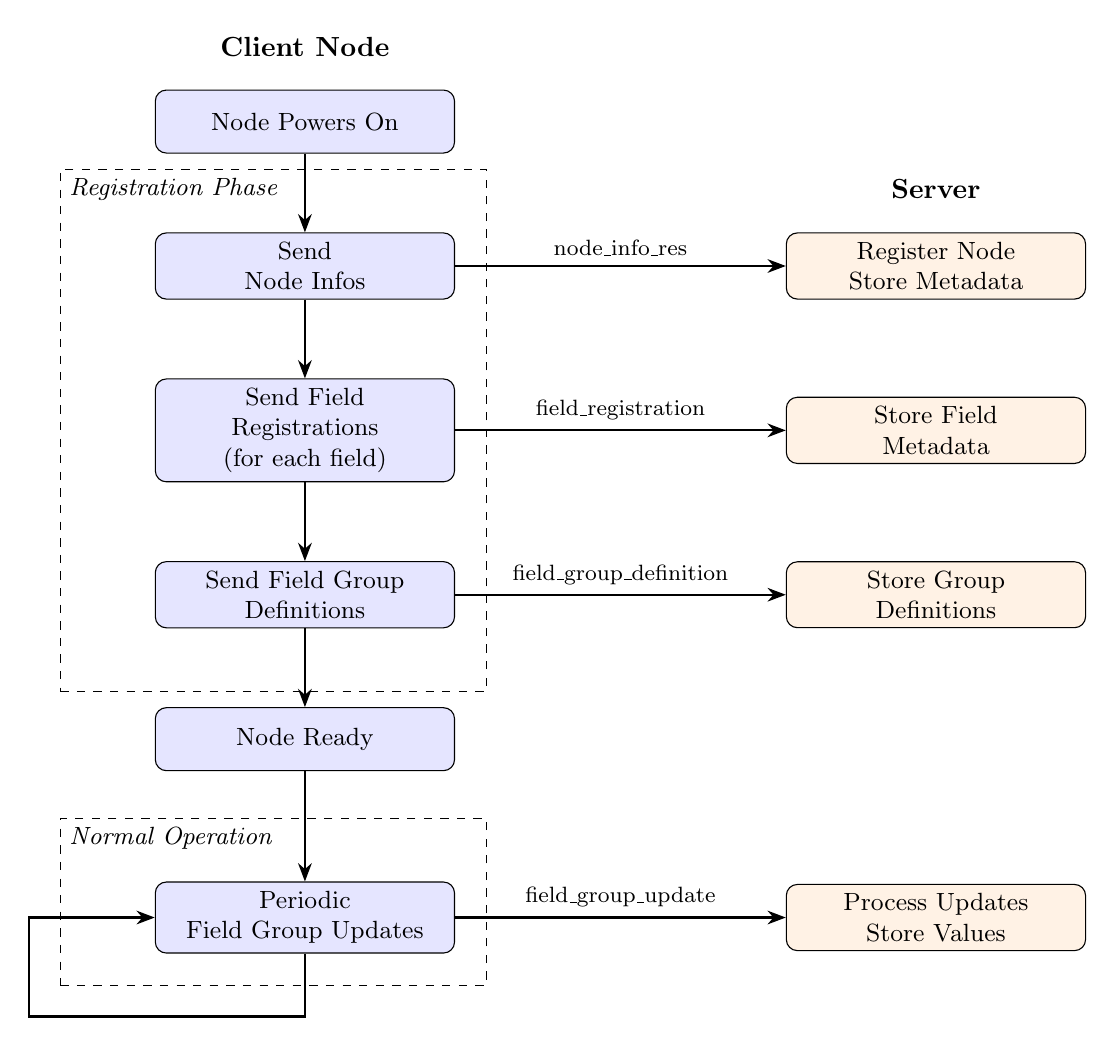
\begin{tikzpicture}[
    node distance=10mm,
    every node/.style={font=\small},
    box/.style={rectangle, draw, rounded corners, minimum width=3.8cm, minimum height=8mm, align=center, fill=blue!10},
    serverbox/.style={rectangle, draw, rounded corners, minimum width=3.8cm, minimum height=8mm, align=center, fill=orange!10},
    arrow/.style={-{Stealth[]}, thick},
    dasharrow/.style={-{Stealth[]}, thick, dashed}
]
    % Node column
    \node[box] (start) {Node Powers On};
    \node[box, below=of start] (sendinfo) {Send\\ Node Infos};
    \node[box, below=of sendinfo] (sendreg) {Send Field\\Registrations\\(for each field)};
    \node[box, below=of sendreg] (sendgroup) {Send Field Group\\Definitions};
    \node[box, below=of sendgroup] (ready) {Node Ready};
    \node[box, below=14mm of ready] (periodic) {Periodic\\Field Group Updates};
    
    % Server column
    \node[serverbox, right=42mm of sendinfo] (rcvinfo) {Register Node\\Store Metadata};
    \node[serverbox, right=42mm of sendreg] (rcvreg) {Store Field\\Metadata};
    \node[serverbox, right=42mm of sendgroup] (rcvgroup) {Store Group\\Definitions};
    \node[serverbox, right=42mm of periodic] (process) {Process Updates\\Store Values};
    
    % Labels
    \node[above=3mm of start, font=\bfseries] {Client Node};
    \node[above=3mm of rcvinfo, font=\bfseries] {Server};
    
    % Arrows - registration phase
    \draw[arrow] (start) -- (sendinfo);
    \draw[arrow] (sendinfo) -- (sendreg);
    \draw[arrow] (sendreg) -- (sendgroup);
    \draw[arrow] (sendgroup) -- (ready);
    \draw[arrow] (ready) -- (periodic);
    
    % Message arrows
    \draw[arrow] (sendinfo.east) -- (rcvinfo.west) node[midway, above, font=\footnotesize] {node\_info\_res};
    \draw[arrow] (sendreg.east) -- (rcvreg.west) node[midway, above, font=\footnotesize] {field\_registration};
    \draw[arrow] (sendgroup.east) -- (rcvgroup.west) node[midway, above, font=\footnotesize] {field\_group\_definition};
    \draw[arrow] (periodic.east) -- (process.west) node[midway, above, font=\footnotesize] {field\_group\_update};
    
    % Phases - asymmetric padding (more on left)
    \node[draw, dashed, fit=(sendinfo) (sendreg) (sendgroup), inner xsep=8mm, inner ysep=8mm, xshift=-4mm] (regphase) {};
    \node[draw, dashed, fit=(periodic), inner xsep=8mm, inner ysep=6mm, xshift=-4mm,yshift=2mm] (opphase) {};
    
    % Phase labels - positioned outside the boxes
    \node[anchor=north west, font=\small\itshape] at (regphase.north west) {Registration Phase};
    \node[anchor=north west, font=\small\itshape] at (opphase.north west) {Normal Operation};
    
    % Loop arrow for periodic updates
    \draw[arrow] (periodic.south) -- ++(0,-8mm) -| ($(periodic.west)+(-16mm,0)$) -- (periodic.west);
    
\end{tikzpicture}
\caption{Field Registration and Update Flow}
\end{figure}

\subsection{Registration}\label{subsec:registration}
Variables and parameters are dynamically defined over the bus.
\paragraph{}
After initializing registration, a node sends out \texttt{field\_registration} messages, one for each 
parameter/variable. The FieldRegistration includes a per-node-unique field ID (parameters and variables can have the same ID on the same node), the datatype of the field, and 
a human-readable name. From this point on, the server knows which types of fields the node has.

\paragraph{}
Next, the node sends \texttt{field\_group\_definition} messages. Variables and parameters cannot be mixed together in one FieldGroupDefinition.
. The node sends a group ID to identify the group and a list of field IDs. The order of the 
field IDs must be the same as the order of fields in future \texttt{field\_group\_updates}. The node must ensure that all of the fields defined can fit into a FieldGroupUpdate.


\subsection{Regular Operation}\label{subsec:regular-operation}
\subsubsection{Field Updates}\label{subsubsec:field-updates}
During regular operation, each node sends \texttt{field\_group\_update} messages at a defined interval. 
The interval can vary between groups, allowing nodes to send fields at different intervals to, for example, reduce bus utilization.

\subsubsection{Parameter Setting}\label{subsubsec:parameter-setting}
Other bus members can send a \texttt{parameter\_set\_req} message, which includes the field ID of the parameter and the new value.
Once the node receives the request, it changes the internal parameter value and responds with a \texttt{parameter\_set\_res} message containing the 
new value. This should be the actual value read back from the parameter, not simply the value that was received in the request.


When a parameter is internally modified through some automated system, the updated value must be sent as a \texttt{parameter\_set\_res} message to the server.
\subsubsection{Parameter Locking}\label{subsubsec:parameter-locking}

A parameter can optionally be locked and later unlocked through a \texttt{parameter\_set\_lock\_req} message (see \ref{struct:ParameterSetLock} and \ref{msg:parameter-set-lock-req}).
After a parameter has been locked, it cannot be modified by an external node.
A parameter can only be unlocked by the locking node or the server. \todo{Is this needed as part of the protocol?}
\paragraph{}
\subsubsection{Requesting Field Data}\label{subsubsec:requesting-field-data}
A field can be accessed through a \texttt{field\_get\_req} message, which contains the field ID.
Nodes respond with a \texttt{field\_get\_res} message, containing the field ID and the value of the field.

\section{Heartbeats}\label{sec:heartbeats}
Heartbeats ensure that the system does not reach a state where it is still dangerous to physically handle but 
not accessible through CAN messages. The \texttt{heartbeat\_req} message sent from the server, contains a continuously increasing counter.
The counter value is unique to each node. If a node does not receive \texttt{heartbeat\_req} messages, it will default
to a safe state. Similarly, the server takes note of any unresponsive nodes.

\section{Status Messages}\label{sec:status-messages}
Nodes may send optional status messages to the server.
Currently, the three status message types are: \texttt{info\_status}, \texttt{warning\_status}, and \texttt{error\_status}, as defined in section~\ref{sec:message-types}.
Each message contains a null-terminated string with a status message.
\section{Message Types}\label{sec:message-types}
The following message types are defined in the protocol:

\begin{center}
\begin{longtable}{c l l p{6cm}}
\toprule
\textbf{Enum} & \textbf{Message Type} & \textbf{Data Payload} & \textbf{Description} \\
\endhead
 
\multicolumn{4}{l}{\textit{Node Discovery and Information}} \\
0 & \texttt{node\_info\_req}\label{msg:node-info-req} & No payload & Request node information \\
1 & \texttt{node\_info\_res}\label{msg:node-info-res} & NodeInfoRes (\ref{struct:NodeInfoRes}) & Response with node capabilities and identification \\
\midrule
\multicolumn{4}{l}{\textit{Status Messages}} \\
10 & \texttt{info\_status}\label{msg:info-status} & Status (\ref{struct:Status}) & Informational status message \\
11 & \texttt{warning\_status}\label{msg:warning-status} & Status (\ref{struct:Status}) & Warning status message \\
12 & \texttt{error\_status}\label{msg:error-status} & Status (\ref{struct:Status}) & Error status message \\
\midrule
\multicolumn{4}{l}{\textit{Field Registration}} \\
20 & \texttt{variable\_registration}\label{msg:variable-registration} & FieldRegistration (\ref{struct:FieldRegistration}) & Register a variable field \\
21 & \texttt{parameter\_registration}\label{msg:parameter-registration} & FieldRegistration (\ref{struct:FieldRegistration}) & Register a parameter field \\
\midrule
\multicolumn{4}{l}{\textit{Field Group Management}} \\
30 & \texttt{field\_group\_definition}\label{msg:field-group-definition} & FieldGroupDefinition (\ref{struct:FieldGroupDefinition}) & Define a group of fields for batch updates \\
31 & \texttt{field\_group\_update}\label{msg:field-group-update} & FieldGroupUpdate (\ref{struct:FieldGroupUpdate}) & Update values for a field group \\
\midrule
\multicolumn{4}{l}{\textit{Heartbeat}} \\
40 & \texttt{heartbeat\_req}\label{msg:heartbeat-req} & HeartBeat (\ref{struct:HeartBeat}) & Heartbeat request \\
41 & \texttt{heartbeat\_res}\label{msg:heartbeat-res} & HeartBeat (\ref{struct:HeartBeat}) & Heartbeat response \\
\midrule
\multicolumn{4}{l}{\textit{Parameter Management}} \\
50 & \texttt{parameter\_set\_req}\label{msg:parameter-set-req} & ParameterSetReq (\ref{struct:ParameterSetReq}) & Request to set a parameter value \\
51 & \texttt{parameter\_set\_res}\label{msg:parameter-set-res} & ParameterSetRes (\ref{struct:ParameterSetRes}) & Response with confirmed parameter value \\
52 & \texttt{parameter\_set\_lock\_req}\label{msg:parameter-set-lock-req} & ParameterSetLock (\ref{struct:ParameterSetLock}) & Request to lock a parameter \\
53 & \texttt{parameter\_set\_lock\_res}\label{msg:parameter-set-lock-res} & ParameterSetLock (\ref{struct:ParameterSetLock}) & Response confirming parameter lock \\
\midrule
\multicolumn{4}{l}{\textit{Field Access}} \\
60 & \texttt{field\_get\_req}\label{msg:field-get-req} & FieldGetReq (\ref{struct:FieldGetReq}) & Request field value \\
61 & \texttt{field\_get\_res}\label{msg:field-get-res} & FieldGetRes (\ref{struct:FieldGetRes}) & Response with field value \\

\bottomrule
\end{longtable}
\end{center}

\section{Data Structures}\label{sec:data-structures}

\subsection{NodeInfoRes}\label{struct:NodeInfoRes}
Response containing information about a node's capabilities.


\begin{figure}[H]
\centering
\begin{bytefield}[
bitwidth=\widthof{liquid\_hash },
leftcurly=., leftcurlyspace=2pt]{8}
\begin{leftwordgroup} {0}
 \bitheader[bitformatting=\large]{0-7} \\
\bitbox{1}{var\_cnt} & \bitbox{1}{par\_cnt} & 
\bitbox{4}{firmware\_hash} &
& &  \bitbox{2}{liquid\_hash  }
\end{leftwordgroup}\\

\begin{leftwordgroup} {1}
\bitbox{2}{liquid\_hash} \bitbox[lrt]{6}{  }
\end{leftwordgroup}\\

\begin{leftwordgroup} {2}
\bitbox[lr]{8}{  }
\end{leftwordgroup}\\
\begin{leftwordgroup} {3}
\bitbox[lr]{8}{  }
\end{leftwordgroup}\\
\begin{leftwordgroup} {4}
\bitbox[lr]{8}{ device name }
\end{leftwordgroup}\\
\begin{leftwordgroup} {5}
\bitbox[lr]{8}{  }
\end{leftwordgroup}\\
\begin{leftwordgroup} {6}
\bitbox[lr]{8}{  }
\end{leftwordgroup}\\
\begin{leftwordgroup} {7}
\bitbox[lrb]{8}{  }
\end{leftwordgroup}\\

\end{bytefield}

\vspace{2mm}


\caption{NodeInfoRes byte layout (8 bytes per row)}
\end{figure}

\textbf{Field Descriptions:}

\begin{center}
\begin{tabular}{l c l}
\toprule
Field & Bytes & Description \\
\midrule
variable\_count & 1 & Number of variables on this node \\
parameter\_count & 1 & Number of parameters on this node \\
firmware\_hash & 4 & Hash of the firmware version \\
liquidcan\_hash & 4 & Hash of the LiquidCan protocol version \\
device\_name & 53 & Human-readable device name \\
\midrule
\textbf{Total} & \textbf{63} & \\
\bottomrule
\end{tabular}
\end{center}

% TODO: Describe the purpose and usage of NodeInfoRes

\begin{lstlisting}[caption={NodeInfoRes struct}]
typedef struct __attribute__((packed)) {
    uint8_t variable_count;
    uint8_t parameter_count;
    uint32_t firmware_hash;
    uint32_t liquidcan_hash;
    char device_name[53];
} node_info_res_t;
\end{lstlisting}

\subsection{Status}\label{struct:Status}
General status message with text information.

\begin{center}
\begin{tabular}{l c l}
\toprule
Field & Bytes & Description \\
\midrule
msg & 63 & Status message text \\
\bottomrule
\end{tabular}
\end{center}

% TODO: Describe when status messages are used

\begin{lstlisting}[caption={Status struct}]
typedef struct __attribute__((packed)) {
    char msg[63];
} status_t;
\end{lstlisting}

\subsection{FieldRegistration}\label{struct:FieldRegistration}
Registration information for a variable or parameter field.
The DataType here refers to the DataType Enum value (see \ref{subsec:DataType}).

\begin{center}
\begin{tabular}{l c l}
\toprule
Field & Bytes & Description \\
\midrule
field\_id & 1 & Unique identifier for this field \\
field\_type & 1 & Data type (DataType enum) \\
field\_name & 61 & Human-readable field name \\
\midrule
\textbf{Total} & \textbf{63} & \\
\bottomrule
\end{tabular}
\end{center}


\begin{lstlisting}[caption={FieldRegistration struct}]
typedef struct __attribute__((packed)) {
    uint8_t field_id;
    uint8_t field_type; 
    char field_name[61];
} field_registration_t;
\end{lstlisting}

\subsection{FieldGroupDefinition}\label{struct:FieldGroupDefinition}
Defines a group of related fields for efficient batch updates.
The 
\begin{center}
\begin{tabular}{l c l}
\toprule
Field & Bytes & Description \\
\midrule
group\_id & 1 & Unique identifier for this group \\
field\_ids & 62 & Array of field IDs in this group \\
\midrule
\textbf{Total} & \textbf{63} & \\
\bottomrule
\end{tabular}
\end{center}

% TODO: Describe field group usage and maximum number of fields per group

\begin{lstlisting}[caption={FieldGroupDefinition struct}]
typedef struct __attribute__((packed)) {
    uint8_t group_id;
    uint8_t field_ids[62];
} field_group_definition_t;
\end{lstlisting}

\subsection{FieldGroupUpdate}\label{struct:FieldGroupUpdate}
Updates all field values in a previously defined group.

\begin{center}
\begin{tabular}{l c l}
\toprule
Field & Bytes & Description \\
\midrule
group\_id & 1 & Group identifier \\
values & 62 & Packed values for all fields in the group \\
\midrule
\textbf{Total} & \textbf{63} & \\
\bottomrule
\end{tabular}
\end{center}

\textbf{Note:} The values are packed in the same order as announced in the FieldGroupDefinition.

% TODO: Describe value packing rules and alignment

\begin{lstlisting}[caption={FieldGroupUpdate struct}]
typedef struct __attribute__((packed)) {
    uint8_t group_id;
    uint8_t values[62];
} field_group_update_t;
\end{lstlisting}

\subsection{HeartBeat}\label{struct:HeartBeat}
Simple heartbeat message with counter.

\begin{center}
\begin{tabular}{l c l}
\toprule
Field & Bytes & Description \\
\midrule
counter & 4 & Incrementing counter value \\
\bottomrule
\end{tabular}
\end{center}

% TODO: Describe heartbeat interval and timeout behavior

\begin{lstlisting}[caption={HeartBeat struct}]
typedef struct __attribute__((packed)) {
    uint32_t counter;
} heartbeat_t;
\end{lstlisting}

\subsection{ParameterSetReq}\label{struct:ParameterSetReq}
Request to set a parameter value.

\begin{center}
\begin{tabular}{l c l}
\toprule
Field & Bytes & Description \\
\midrule
parameter\_id & 1 & Parameter identifier \\
value & 62 & New value (type depends on parameter) \\
\midrule
\textbf{Total} & \textbf{63} & \\
\bottomrule
\end{tabular}
\end{center}

\begin{lstlisting}[caption={ParameterSetReq struct}]
typedef struct __attribute__((packed)) {
    uint8_t parameter_id;
    uint8_t value[62];
} parameter_set_req_t;
\end{lstlisting}

\subsection{ParameterSetRes}\label{struct:ParameterSetRes}
Response to a parameter set request.

\begin{center}
\begin{tabular}{l c l}
\toprule
Field & Bytes & Description \\
\midrule
parameter\_id & 1 & Parameter identifier \\
value & 62 & Confirmed value after set operation \\
\midrule
\textbf{Total} & \textbf{63} & \\
\bottomrule
\end{tabular}
\end{center}


\begin{lstlisting}[caption={ParameterSetRes struct}]
typedef struct __attribute__((packed)) {
    uint8_t parameter_id;
    uint8_t value[62];
} parameter_set_res_t;
\end{lstlisting}

\subsection{FieldGetReq}\label{struct:FieldGetReq}
Request to retrieve a field value.
Parameters are symbolized by field\_type = 0 and variables by field\_type = 1.
\begin{center}
\begin{tabular}{l c l}
\toprule
Field & Bits/Bytes & Description \\
\midrule
field\_type & 1 bit & Type of field(parameter or variable) \\
field\_id & 1 Byte & Field identifier \\
\bottomrule
\end{tabular}
\end{center}

% TODO: Describe field retrieval process

\begin{lstlisting}[caption={FieldGetReq struct}]
typedef struct __attribute__((packed)) {
    uint8_t field_id : 1;
    uint8_t field_id : 8;
} field_get_req_t;
\end{lstlisting}

\subsection{FieldGetRes}\label{struct:FieldGetRes}
Response with requested field value.

\begin{center}
\begin{tabular}{l c l}
\toprule
Field & Bytes & Description \\
\midrule
field\_id & 1 & Field identifier \\
value & 62 & Field value \\
\midrule
\textbf{Total} & \textbf{63} & \\
\bottomrule
\end{tabular}
\end{center}

% TODO: Describe response format

\begin{lstlisting}[caption={FieldGetRes struct}]
typedef struct __attribute__((packed)) {
    uint8_t field_id;
    uint8_t value[62];
} field_get_res_t;
\end{lstlisting}

\subsection{ParameterSetLock}\label{struct:ParameterSetLock}
Locks a parameter to prevent changes.

\begin{center}
\begin{tabular}{l c l}
\toprule
Field & Bytes & Description \\
\midrule
parameter\_id & 1 & Parameter identifier to lock \\
\bottomrule
\end{tabular}
\end{center}

% TODO: Describe parameter locking mechanism and use cases

\begin{lstlisting}[caption={ParameterSetLock struct}]
typedef struct __attribute__((packed)) {
    uint8_t parameter_id;
} parameter_set_lock_t;
\end{lstlisting}


\subsection{DataType}\label{subsec:DataType}
The protocol supports the following data types:
\begin{center}
\begin{tabular}{l l l}
\toprule
Enum Values & Type Name & Description \\
\midrule
0 & \texttt{Float32} & 32-bit floating point \\
1 & \texttt{Int32} & 32-bit signed integer \\
2 & \texttt{Int16} & 16-bit signed integer \\
3 & \texttt{Int8} & 8-bit signed integer \\
4 & \texttt{UInt32} & 32-bit unsigned integer \\
5 & \texttt{UInt16} & 16-bit unsigned integer \\
6 & \texttt{UInt8} & 8-bit unsigned integer \\

\bottomrule
\end{tabular}
\end{center}

\section{Versioning and Extension Mechanisms}\label{sec:versioning}
% TODO: Describe:
% - Version tracking using firmware_hash and liquidcan_hash
% - Protocol versioning strategy
% - Backwards compatibility rules
% - How to handle unknown message types
This protocol uses semantic versioning.
See \href{https://semver.org/}{https://semver.org/} for a detailed description. A minor update version would, for example, be adding a new datatype or a new message type . Every update of the document must trigger an update of the liquidCAN repo, containing the Rust and C code for each implementation. The updated repo must be reflected in the \texttt{liquidcan\_hash} field of the \texttt{node\_info\_res} used in the firmware/server.

\end{document}